\chapter{Analysis}

\section{Introduction}

\subsection{Client Identification}
My client is Susannah Mason, she is 50 years old and has little usage of computers, except when having to order new stock for the pharmacy. currently the pharmacy uses computerised methods to submit orders to the warehouse.

Suesannah is a pharmacutical manager at spire healthcare in impington 

by  creating this program it would speed up the process making leeping track of and ordering of new equipment and stock alot easier for her 
\subsection{Define the current system}
 the current system uses mostly computer based order submission and price checks but the orders have to be put through the computer manually 
\subsection{Describe the problems}
the orders for the stock take too long to submit and all stock has to be conted by hand 
\pagebreak{}
\subsection{Section appendix}

\begin{figure}[ht!]
\centering
\includegraphics[trim = 7mm 300mm 0mm 70mm, clip, width=140mm, scale=2]{questionaire.JPG}
\caption{questionaire \label{overflow}}
\end{figure}
\pagebreak{}
\section{Investigation}
\subsection{The current system}
the current system at the pharmacy is a data base that holds the information of over 500 items. the data base holds the price the mass the desription and how much is in the pharmacy at that point in time. when an item is taken out of stock the pharmacist has a card to say that an item has been removed from the storage cupboard. sometimes the system deosn't update even when the card is swiped to say a product has been removed
\subsubsection{Data sources and destinations}
\begin{table}[h]
\begin{tabular}{|c|c|c|}
\hline
Data Source & Travels via & destination\\
\hline
doctor & gives prescription & patient\\
\hline
patient & requests medicine & pharmacist\\
\hline
pharmacist & checks stock & stock system\\
\hline 
stock system & gives information & pharmasict\\
\hline
pharmacist & collects medication & medicine cupboard\\
\hline
pharmacist & gives medicine & patient\\
\hline
\end{tabular}
\caption{}
\label{tab:}
\end{table}

\subsubsection{Algorithms}
i will be using quite a few algorithums for this assignment
\begin{algorithm}
    \caption{if statement}
\begin{algorithmic}[1]
\For{$item\ to\ check = 0\ to\ 50$}
	\If{$item = lowest\ minimum\ amount$}
		\State{$"you\ don't\ need\ any\ more\ tablets"$}
	\Else
		\State{$"you\ need\ more\ tablets"$}
	\EndIf
\EndFor
\end{algorithmic}
\end{algorithm}

this other algorithm will be used to calculate the exact price of all of the order 
\begin{algorithm}[h]
\begin{algorithmic}[1]
\If{$order\ Submitted = True$}
	\State{$calculate\ Order$}
\Else
	\State{$Restart\ stock\ check$}
\EndIf
\end{algorithmic}
\end{algorithm}

using the information in the list Items the exact price is calulated
\begin{algorithm}[h]
\begin{algorithmic}[1]
\If{$item\ in\ items = True$}
	\State{$total \gets total\ +\ itemPrice$}
\Else
	\State{$total \gets total$}
\EndIf
\end{algorithmic}
\end{algorithm}

\subsubsection{Data flow diagram}
\begin{figure}[ht!]
\centering
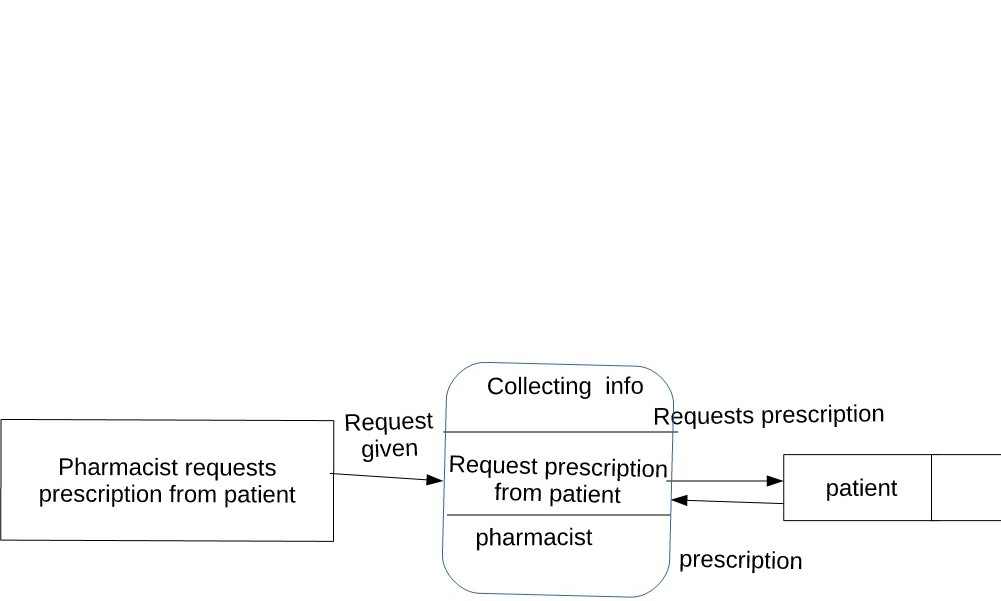
\includegraphics[trim = 0mm 0mm 0mm 5cm , clip, width=130mm]{dfd.JPG}
\end{figure}
\begin{figure}[ht!]
\centering
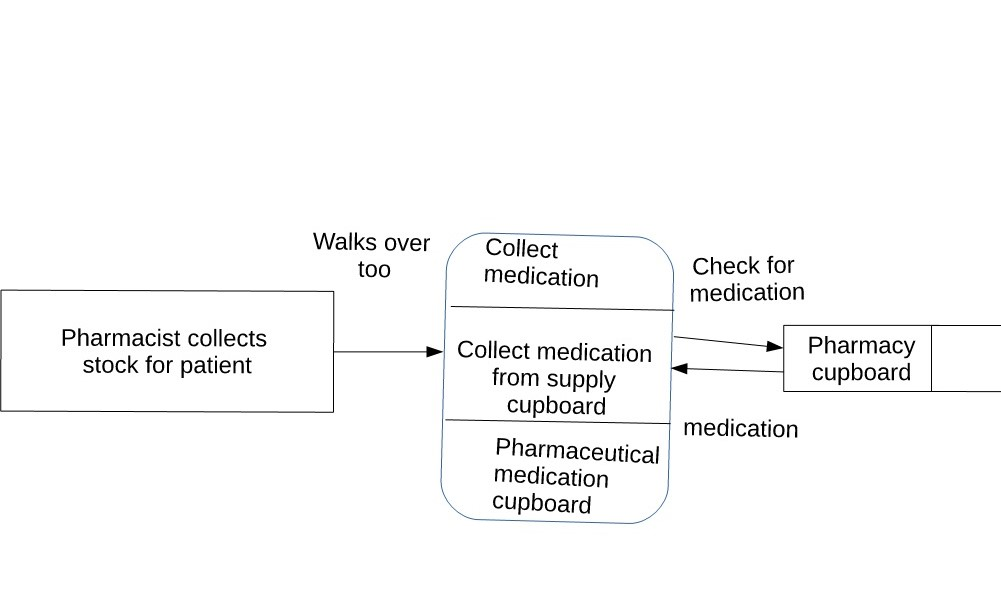
\includegraphics[trim = 0mm 0mm 0mm 5cm , clip, width=130mm]{dfd3.JPG}
\end{figure}
\pagebreak
\subsubsection{Input Forms, Output Forms, Report Formats}
\begin{figure}[ht!]
\centering
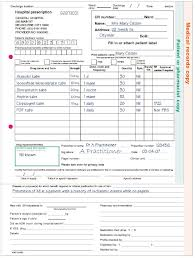
\includegraphics[scale = 1.5]{hospital pres.JPG}
\end{figure}
\pagebreak
\subsection{The proposed system}
the proposed system will be used to order, check stock and be informed as soon as anything leaves the pharmacy the data base will be updated of the removal, as well as if the product falls below a certain point it will be program to replace the stock by ordering new stock form the wearhouse automatically but the order will go through a master contol point before being sent off 
\subsubsection{Data sources and destinations}
\begin{table}[h]
\begin{tabular}{|c|c|c|}
\hline
Data Source & Travels via & destination\\
\hline
doctor & sends email & pharmacy\\
\hline
pharmacist & checks stock & stock system\\
\hline 
stock system & gives information & pharmasict\\
\hline
pharmacist & collects medication & medicine cupboard\\
\hline
patient & collects from & pharmacy\\
\hline
\end{tabular}
\end{table}
\pagebreak
\subsubsection{Data flow diagram}
\begin{figure}[ht!]
\centering
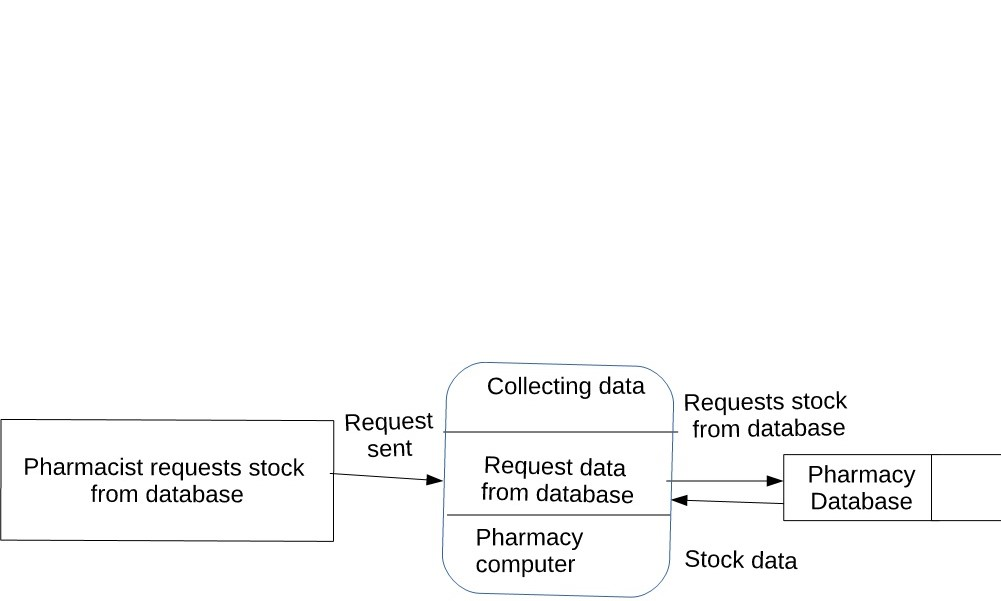
\includegraphics[trim = 0mm 0mm 0mm 5cm , clip, width=130mm]{dfd2.JPG}
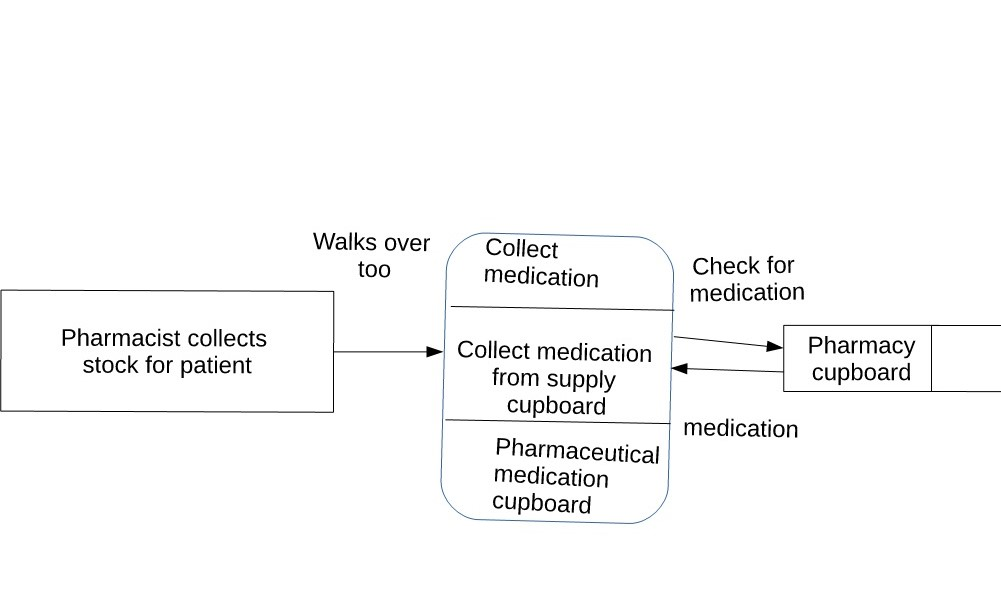
\includegraphics[trim = 0mm 0mm 0mm 5cm , clip, width=130mm]{dfd3.JPG}
\caption{data flow diagram \label{overflow}}
\end{figure}
\subsubsection{Data dictionary}
\begin{table}[h]
\begin{tabular}{|c|c|c|c|}
\hline
Data & Uses & Name \\
\hline
stock detail & stock number & stock check\\
\hline
prescription information & mediction needed & prescription\\
\hline
enough item in stock False & order more item & update stock\\
\hline
\end{tabular}
\label{table:nonlin}
\end{table}

\subsubsection{Volumetrics}
this system should only be used by pharmacutical staff in hospitals my client uses this system normally after every patient has gone through to update the stock. so my predicted amount of memory used by the system should calculate upt around 64 bytes to 256 bytes.
\section{Objectives}
\subsection{General Objectives}
\begin{itemize}
	\item to make a stable system that checks, updates, restocks and sends payment for the ordered items
	\item to give the system to auto restock items when they fall below a certain number of items
	\item to graph which items are being bought or used faster and updates the resocking system acordingly 
\end{itemize}
\subsection{Specific Objectives}
\begin{itemize}
	\item to design a program that will make sorting through the items at the pharmacy as well as store the price and item location in the pharmacy as well as the amount.
\end{itemize}
\subsection{Core Objectives}
\begin{itemize}
\item self updating stock system
\item easy accessablilty
\item order more items to refill stock
\end{itemize}
\subsection{Other Objectives}
\begin{itemize}
    \item the stock keeping on the program should be accurate. E.G. showing how much on tablet of paracitamol costs
    \item the system must have a automatic communication between the wholesale (warehouse) and the pharmacy
\end{itemize}
\section{ER Diagrams and Descriptions}
\subsection{ER Diagram}
\begin{figure}[ht!]
\centering
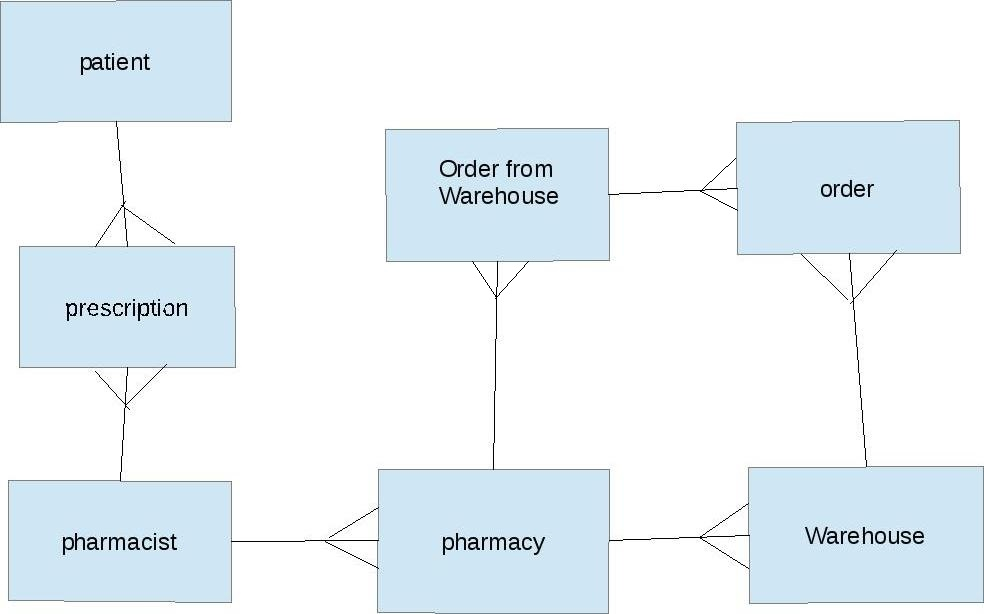
\includegraphics[width=110mm]{table1.JPG}
\caption{entity relationship diagram \label{overflow}}
\end{figure}
\pagebreak
\subsection{Entity Descriptions}
\begin{itemize}
\item Client(\underline{clientID}, PharmacyNum, surname, FirstName, PhoneNumber, Address,Postcode)
\item Pharmacist(\underline{PharamacistID},\emph{PharmacyNum},Surname,FirstName,PhoneNumber,Address,Email)
\item Pharmacy(\underline{PharmacyNum},PharmacyAddress,PharmacyPhoneNumber)
\item Warehouse(\underline{WareHouseNum},\emph{PharmacyAddress},WareHouseAddress)
\item Order(\underline{OrderNum},\emph{WareHouseNum},\emph{PharmacyLocation},OrderDate,size)
\end{itemize}
\section{Object Analysis}
\begin{figure}[ht!]
\centering
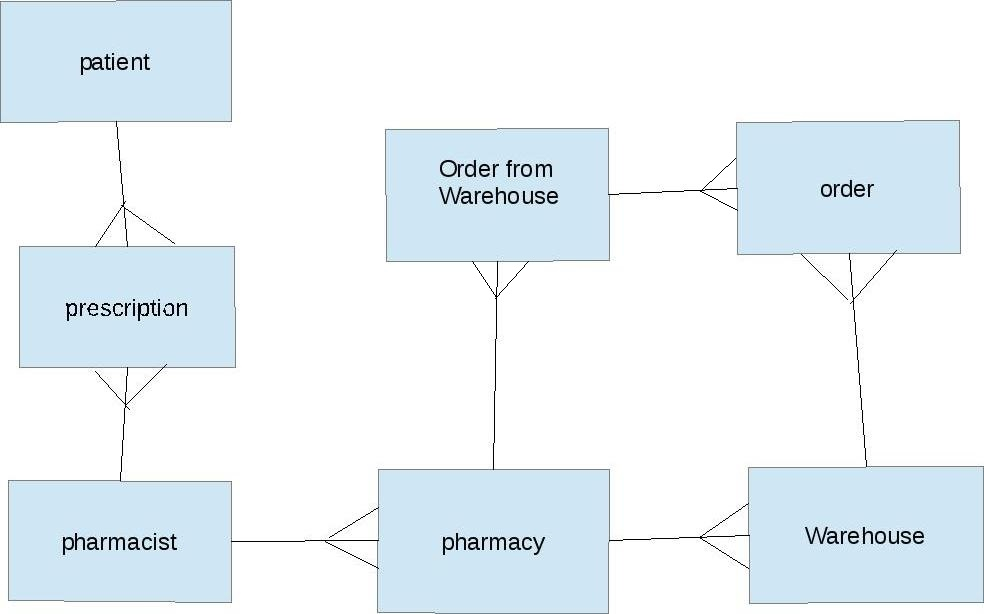
\includegraphics[width=110mm]{table1.JPG}
\caption{entity relationship diagram \label{overflow}}
\end{figure}
\subsection{Object Listing}
\begin{itemize}

\item Client
\item Pharmacist
\item Pharmacy
\item Warehouse
\item Order

\end{itemize}
\subsection{Relationship diagrams}
\begin{figure}[ht!]
\centering
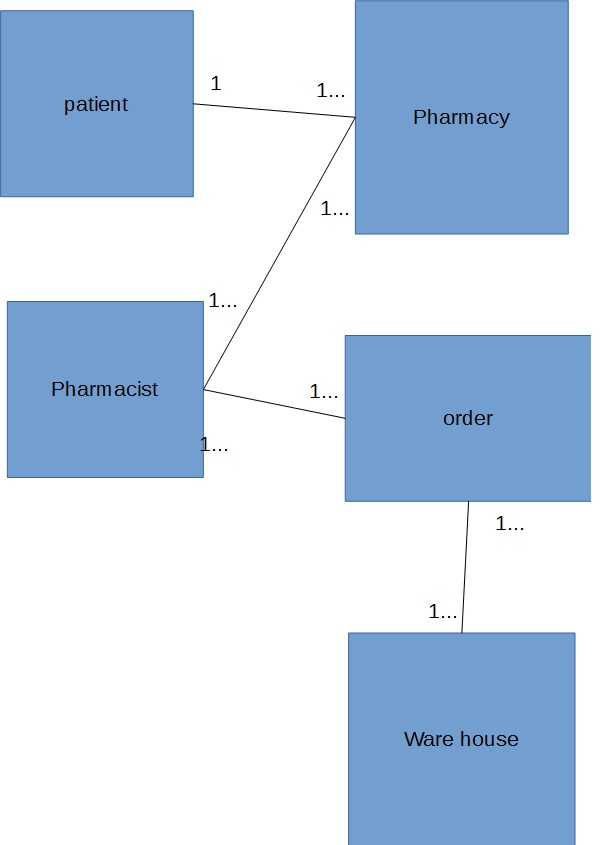
\includegraphics[width=110mm]{er diagram.JPG}
\end{figure}
\subsection{Class definitions}
\begin{table}[h]
\begin{tabular}{|l|}
\hline
hospital member\\
\hline
Surname\\
Firstname\\
Phone Number\\
address\\
\hline
\\
\hline
\end{tabular}
\begin{tabular}{|l|}
\hline
pharmacist: hospital member\\
\hline
\textbf{not inherited:}\\
\underline{PharmacistID}\\
\emph{PharmacyNum}\\
email\\
\textbf{inherited:}\\
Surname\\
Firstname\\
Phone Number\\
address\\
\hline
\end{tabular}
\begin{tabular}{|l|}
\hline
patient: hospital member\\
\hline
\textbf{not inherited:}\\
\underline{ClientID}\\
\emph{PharmacyNum}\\
Postcode\\
\textbf{inherited:}\\
Surname\\
Firstname\\
Phone Number\\
address\\
\hline
\\
\hline
\end{tabular}
\begin{tabular}{|r|}
\hline
Warehouse\\
\hline
\textbf{not inherited:}\\
\underline{WareHouseNum}\\
\emph{PharmacyAddress}\\
WareHouseAddress\\
\hline
\\
\hline
\end{tabular}
\begin{tabular}{|r|}
\hline
Pharmacy\\
\hline
\textbf{not inherited:}\\
\underline{Pharmacynum}\\
PharmacyAddress\\
PharmacyPhoneNumber\\
\hline
\\
\hline
\end{tabular}
\begin{tabular}{|r|}
\hline
Order\\
\hline
\textbf{not inherited:}\\
\underline{OrderNum}\\
OrderDate\\
SizeOfOrder\\
\textbf{inherited:}\\
\emph{WareHouseNum}\\
\emph{PharmacyAddress}\\
\hline
\\
\hline
\end{tabular}
\label{tab:nonlin}
\end{table}
\section{Constraints}
\subsection{Hardware}
Susannah uses a small laptop computer. the components of that laptop are listed below:  
\begin{itemize}
\item 10.1" display
\item intel core N270 atom 1.6 ghz
\item 1.00GB DDR3 RAM
\item 160GB HDD 
\end{itemize}
The proposed system should work on this laptop because of the laptops fast processor it will run through the calculations fast enough.

If using the laptop doesn't work i will switch back to my desktop computer which has:
 \begin{itemize}
\item 17" display 1024 x 768 pixels
\item 34" display 1360 x 768 pixels
\item amd A6-3500 APU 3.0 ghz
\item 4.00GB DDR3 RAM
\item 0.5TB HDD 
\end{itemize}
There should be no problems running the program on this computer.
\subsection{Software}
The operating system used on the laptop is windows xp.
Whereas the operating system used on the desktop is running windows 7.
The programs that i will be using will be python 3.2.
\subsection{Time}
The final submission of the implimentation of the program must be in by the 13th of February 
\subsection{User Knowledge}
The system i will be building will require at least a little background into the pharmacutical area. This is due to some of the medicines in the system do not have abbreviated names. The installation should take about 5 to 10 minutes. 
\subsection{Access restrictions}
the proposed system should only be accessable and privileges to the people in pharmacy, as well as the system should be password protectedto ensure no body outside the system can access the stock information.
\space

\section{Limitations}
\subsection{Areas which will not be included in computerisation}
the prescriptions are not given in electronic format so when the patients come to the pharmacy to collect there medicine it has to be collected by the pahrmacists once the patient has got to the pharmacy
\subsection{Areas considered for future computerisation}
the prescriptions should be sent by the doctors to the pharmacy before the patient leaves the doctor so the pharmacy have time to prepare for the patient so they can pick up there prescription and pay and leave all within the space of one minute.
\pagebreak
\section{Solutions}
\subsection{Alternative solutions}
\begin{table}[h]
\begin{tabular}{|p{4cm}|p{4cm}|p{4cm}|}
\hline
solution & advantages & disadvantages\\
\hline
created program that checks the stock after an item is removed & this will keep a continually accurate stock check & this will take up more space to program in\\
\hline
&&\\
\hline
\end{tabular}
\caption{}
\label{tab:nonlin}
\end{table}

\subsection{Justification of chosen solution}
I have chosen to the Python 3.2 desktop application with a GUI and SQL' solution. My reason for using this method is:
\begin{itemize}
    \item the application will be specific for pharmacy which will be updated at the start of every week and will continuously keep track of the database where the old system.
    \item the database used will take up less space required to store the data.
    \item due to the databases size making back ups is very easy so if the system.
\end{itemize} 
